\documentclass{report}

\input{preamble}
\input{macros}
\input{letterfonts}

\usepackage{tikz}
\usepackage{tikz-3dplot}
\usepackage{amsmath}
\usepackage{amssymb}
\usepackage{pgfplots}
\usepackage{smartdiagram}
\usepackage{xcolor}
\usepackage{forest}
\usepackage{tikz-3dplot}
\usepgfplotslibrary{colormaps}
\usepgfplotslibrary{groupplots}
\pgfplotsset{compat=newest}

\usesmartdiagramlibrary{additions}

\title{\Huge{Temporary Doc}\\Calc 3}
\author{\huge{Giacomo Cappelletto}}
\date{23/10/24}

\begin{document}


\maketitle
\newpage
\pdfbookmark[section]{\contentsname}{toc}
\tableofcontents
\pagebreak

\chapter{Vector Valued Functions $f:\mathbb{R} \rightarrow \mathbb{R}^n$}


\section{Absolute Extrema}

For a function \( f \) defined on a region \( R \) in \( \mathbb{R}^2 \), a point \( (a, b) \) in \( R \) is an \emph{absolute maximum} of \( f \) if \( f(a, b) \geq f(x, y) \) for any \( (x, y) \) in \( R \). Similarly, \( (a, b) \) is an \emph{absolute minimum} if \( f(a, b) \leq f(x, y) \) for any \( (x, y) \) in \( R \).

\thm{Extreme Value Theorem}{
	If \( R \) is closed and bounded, and if \( f \) is continuous on \( R \), then the absolute extrema of \( f \) on \( R \) can be found by examining:
	\begin{enumerate}
		\item Critical points of \( f \) (for local extrema within \( R \)),
		\item Boundary values of \( f \) on \( R \).
	\end{enumerate}
}

\ex{Example Extreme Value Theorem}{
	Consider the function \( V(\ell, w) = \ell w (96 - \ell - w) \), where \( R = \{ (\ell, w) \mid \ell \geq 0, w \geq 0, \ell + w \leq 96 \} \).

	\begin{enumerate}
		\item Since \( R \) is closed, we can apply the Extreme Value Theorem:
		      \begin{enumerate}
			      \item Find local maxima by setting \( \nabla V(\ell, w) = 0 \).
			      \item Evaluate \( V \) on the boundary of \( R \).
		      \end{enumerate}
	\end{enumerate}

	To find critical points:
	\[
		V(\ell, w) = \ell w (96 - \ell - w)
	\]
	The partial derivatives are:
	\[
		\frac{\partial V}{\partial \ell} = w(96 - 2\ell - w), \quad \frac{\partial V}{\partial w} = \ell(96 - \ell - 2w)
	\]
	Setting these to zero, we get:
	\[
		\begin{cases}
			w(96 - 2\ell - w) = 0 \\
			\ell(96 - \ell - 2w) = 0
		\end{cases}
	\]
	This yields critical points at \( (\ell, w) = (32, 32) \).\\

	On the boundary of \( R \):
	\begin{enumerate}
		\item \( \ell = 0 \): Then \( V = 0 \) for any \( w \).
		\item \( w = 0 \): Then \( V = 0 \) for any \( \ell \).
		\item \( \ell + w = 96 \): Substitute \( w = 96 - \ell \) into \( V(\ell, w) = \ell (96 - \ell) (96 - \ell - (96 - \ell)) = \ell(96 - \ell)^2 \).
	\end{enumerate}

	\begin{center}
		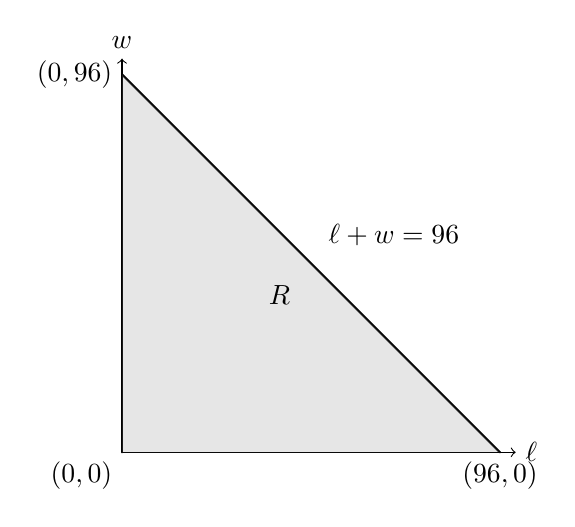
\begin{tikzpicture}[scale=0.05]
			% Draw the axes
			\draw[->] (0, 0) -- (100, 0) node[right] {\( \ell \)};
			\draw[->] (0, 0) -- (0, 100) node[above] {\( w \)};

			% Draw the boundary line l + w = 96
			\draw[thick] (0,96) -- (96,0);
			\node[above right] at (50, 50) {\( \ell + w = 96 \)};

			% Label points
			\filldraw[black] (96,0) circle (1.5pt) node[below] {\( (96, 0) \)};
			\filldraw[black] (0,96) circle (1.5pt) node[left] {\( (0, 96) \)};
			\filldraw[black] (0,0) circle (1.5pt) node[below left] {\( (0, 0) \)};

			% Shade the feasible region
			\fill[gray, opacity=0.2] (0, 0) -- (0, 96) -- (96, 0) -- cycle;

			% Label the region
			\node at (40, 40) {\( R \)};
		\end{tikzpicture}
	\end{center}

	Solving this, we find that \( V(32, 32) = 32 \cdot 32 \cdot 32 = 32768 \), which is the maximum value on \( R \).\\

	To confirm the local maximum at \( (32, 32) \), we compute the Hessian:
	\[
		H(\ell, w) = \begin{bmatrix} -2w & 96 - \ell - w \\ 96 - \ell - w & -2\ell \end{bmatrix}
	\]
	At \( (32, 32) \), the Hessian determinant is:
	\[
		\det(H) = (-2 \times 32)^2 - (96 - 32 - 32)^2 = (64 \times 64) - (32 \times 32) = 32768 > 0
	\]
	Thus, \( V(\ell, w) \) has a local maximum at \( (32, 32) \).
}
\ex{Another Example}{
	Consider \( f(x, y) = 4 - x^2 - y^2 \) on \( R = \{ (x, y) \mid -1 \leq x \leq 1, x^2 + y^2 < 1 \} \). Here, \( R \) is an open region without boundaries.\\

	The maximum of \( f(x, y) \) occurs at \( (0, 0) \), where \( f(0, 0) = 4 \). There is no absolute minimum because for points approaching the boundary (e.g., \( x \approx 0.99 \)), \( f(x, y) \) approaches \( -\infty \).

	Thus, in \( R \), there is no absolute minimum value for \( f \), illustrating the importance of the region's closedness and boundedness for the Extreme Value Theorem to apply.
}

\section{Lagrange Multiplier Method}

\subsection{General Procedure}

To maximize or minimize \( f(x, y) \) subject to a constraint \( g(x, y) = 0 \), follow these steps:

\begin{enumerate}
	\item \textbf{Identify Critical Points:} A point \( (x', y') \) is a critical point if:
	      \begin{itemize}
		      \item There exists \( \lambda \in \mathbb{R} \) such that \( \nabla f(x', y') = \lambda \nabla g(x', y') \) (using the \emph{method of Lagrange multipliers}).
		      \item \( g(x', y') = 0 \).
	      \end{itemize}

	\item \textbf{Evaluate Cases for Critical Points:}
	      \begin{enumerate}
		      \item \textbf{Case 1:} The constraint region \( R \) is bounded and has no endpoints.
		            \begin{itemize}
			            \item In this case, assuming continuity of \( f \), any local extrema within \( R \) are also absolute extrema.
			            \item Select critical points \( (x', y') \) and evaluate \( f \) at these points.
		            \end{itemize}

		      \item \textbf{Case 2:} The constraint region \( R \) is bounded and has endpoints.
		            \begin{itemize}
			            \item Example: \( x^2 - 4y^2 \leq 0 \) with \( -1 \leq x \leq 1 \).
			            \item Absolute extrema may occur at local extrema or endpoints.
			            \item Check critical points and also evaluate \( f \) at the boundary endpoints.
		            \end{itemize}

		      \item \textbf{Case 3:} The constraint region \( R \) is unbounded or does not include all endpoints.
		            \begin{itemize}
			            \item Example: \( x^2 - 4y^2 \) unbounded or \( x^2 + y^2 - 4 = 0 \) with \( -2 \leq x \leq 2 \).
			            \item It may be possible that absolute extrema do not exist.
			            \item Find any critical points and evaluate \( f(x) \) as \( x \rightarrow \pm \infty \) if applicable.
		            \end{itemize}
	      \end{enumerate}
\end{enumerate}

\ex{Lagrange Multiplier Method}{
	We aim to find the absolute extrema of the function \( f(x, y) = x - 2y \) subject to the constraint \( g(x, y) = x^2 + y^2 = 4 \).\\
	To find the extrema, we use the method of Lagrange multipliers, where we seek points where \( \nabla f = \lambda \nabla g \).

	The gradients of \( f \) and \( g \) are:
	\[
		\nabla f(x, y) = \begin{bmatrix} 1 \\ -2 \end{bmatrix}, \quad \nabla g(x, y) = \begin{bmatrix} 2x \\ 2y \end{bmatrix}
	\]
	Setting \( \nabla f = \lambda \nabla g \), we have:
	\[
		\begin{cases}
			1 = \lambda \cdot 2x \\
			-2 = \lambda \cdot 2y
		\end{cases}
	\]
	This simplifies to:
	\[
		\lambda = \frac{1}{2x} = \frac{-1}{y} \Rightarrow y = -2x
	\]

	Substitute \( y = -2x \) into the constraint \( g(x, y) = x^2 + y^2 = 4 \):
	\[
		x^2 + (-2x)^2 = 4 \Rightarrow x^2 + 4x^2 = 4 \Rightarrow 5x^2 = 4 \Rightarrow x = \pm \frac{2}{\sqrt{5}}
	\]
	Then, \( y = -2x \) gives \( y = \pm \frac{4}{\sqrt{5}} \). So the points are:
	\[
		\left( \frac{2}{\sqrt{5}}, -\frac{4}{\sqrt{5}} \right) \quad \text{and} \quad \left( -\frac{2}{\sqrt{5}}, \frac{4}{\sqrt{5}} \right)
	\]

	Calculate \( f(x, y) \) at the points:
	\[
		f\left( \frac{2}{\sqrt{5}}, -\frac{4}{\sqrt{5}} \right) = \frac{2}{\sqrt{5}} + \frac{8}{\sqrt{5}} = \frac{10}{\sqrt{5}} = 2\sqrt{5}
	\]
	\[
		f\left( -\frac{2}{\sqrt{5}}, \frac{4}{\sqrt{5}} \right) = -\frac{2}{\sqrt{5}} - \frac{8}{\sqrt{5}} = -\frac{10}{\sqrt{5}} = -2\sqrt{5}
	\]
	Thus, the \textbf{absolute maximum} is \( 2\sqrt{5} \) and the \textbf{absolute minimum} is \( -2\sqrt{5} \).\\

	Below is a diagram showing the constraint \( x^2 + y^2 = 4 \) as a circle and the level curves of \( f(x, y) = x - 2y \), specifically showing the two tangent level curves at \( z = \pm \frac{10}{\sqrt{5}} \) that represent the maximum and minimum values.

	\begin{center}
		\begin{tikzpicture}[scale=1.5]
			% Draw the constraint circle x^2 + y^2 = 4
			\draw[thick] (0,0) circle (2);
			\node at (2.2, 0) {\( x^2 + y^2 = 4 \)};

			% Draw the level curves of f(x, y) = x - 2y
			\draw[dashed, domain=-2:2] plot({\x}, {(\x - 10/sqrt(5))/2});
			\node[above right] at (1.788854382, -2) {\( x - 2y = \frac{10}{\sqrt{5}} \)};

			\draw[dashed, domain=-2:2] plot({\x}, {(\x + 10/sqrt(5))/2});
			\node[below right] at (1.788854382, 2) {\( x - 2y = -\frac{10}{\sqrt{5}} \)};

			% Draw the points of maximum and minimum
			\filldraw[black] (0.894427191, -1.788854382) circle (0.05);
			\node[below right] at (0.894427191, -1.788854382) {\( \left( \frac{2}{\sqrt{5}}, -\frac{4}{\sqrt{5}} \right) \)};

			\filldraw[black] (-0.894427191, 1.788854382) circle (0.05);
			\node[above left] at (-0.894427191, 1.788854382) {\( \left( -\frac{2}{\sqrt{5}}, \frac{4}{\sqrt{5}} \right) \)};
		\end{tikzpicture}
	\end{center}
}

\ex{Example: Finding Extrema of \( f(x, y) = e^{x+y} \) with Constraint}{
	Consider maximizing or minimizing \( f(x, y) = e^{x+y} \) subject to the constraint \( g(x, y) = x^2 + xy + y^2 - 9 = 0 \).

	\begin{enumerate}
		\item Using the method of Lagrange multipliers, we set up the system:
		      \[
			      \nabla f(x, y) = \lambda \nabla g(x, y)
		      \]
		      which gives:
		      \[
			      \begin{cases}
				      e^{x+y} = \lambda (2x + y) \\
				      e^{x+y} = \lambda (x + 2y)
			      \end{cases}
		      \]

		\item Dividing the equations, we get:
		      \[
			      \frac{2x + y}{x + 2y} = 1 \Rightarrow x = y
		      \]
		\item Substitute \( x = y \) into the constraint \( x^2 + xy + y^2 = 9 \):
		      \[
			      x^2 + x^2 + x^2 = 9 \Rightarrow 3x^2 = 9 \Rightarrow x = \pm \sqrt{3}, \quad y = \pm \sqrt{3}
		      \]
		\item The critical points are \( ( \sqrt{3}, \sqrt{3} ) \) and \( ( -\sqrt{3}, -\sqrt{3} ) \).

		\item Evaluating \( f(x, y) \) at these points:
		      \[
			      f(\sqrt{3}, \sqrt{3}) = e^{2\sqrt{3}}, \quad f(-\sqrt{3}, -\sqrt{3}) = e^{-2\sqrt{3}}
		      \]

		\item Thus, the maximum value is \( e^{2\sqrt{3}} \) and the minimum value is \( e^{-2\sqrt{3}} \).
	\end{enumerate}
}

\ex{Example: Finding Extrema of \( f(x, y) = x - y \) with Constraint}{
	Consider the function \( f(x, y) = x - y \) with the constraint \( g(x, y) = x^2 + y^2 - 3 x y - 20 = 0 \).

	\begin{enumerate}
		\item The gradients are:
		      \[
			      \nabla f(x, y) = \begin{bmatrix} 1 \\ -1 \end{bmatrix}, \quad \nabla g(x, y) = \begin{bmatrix} 2x - 3y \\ 2y - 3x \end{bmatrix}
		      \]

		\item Set \( \nabla f = \lambda \nabla g \):
		      \[
			      \begin{cases}
				      1 = \lambda (2x - 3y) \\
				      -1 = \lambda (2y - 3x)
			      \end{cases}
		      \]

		\item Solving this system, we find critical points at \( (2, -2) \) and \( (-2, 2) \).

		\item Evaluating \( f(x, y) \) at these points:
		      \[
			      f(2, 1) = 1, \quad f(-2, -1) = -1
		      \]

		\item Therefore, the maximum value is \( 1 \) and the minimum value is \( -1 \).
	\end{enumerate}

	By observing the level curves diagram, we can see that the given points do not maximise/minimise the function, as any other line where \( x-y < \pm 4 \) would further increase/decrease the function.

}

\begin{center}
	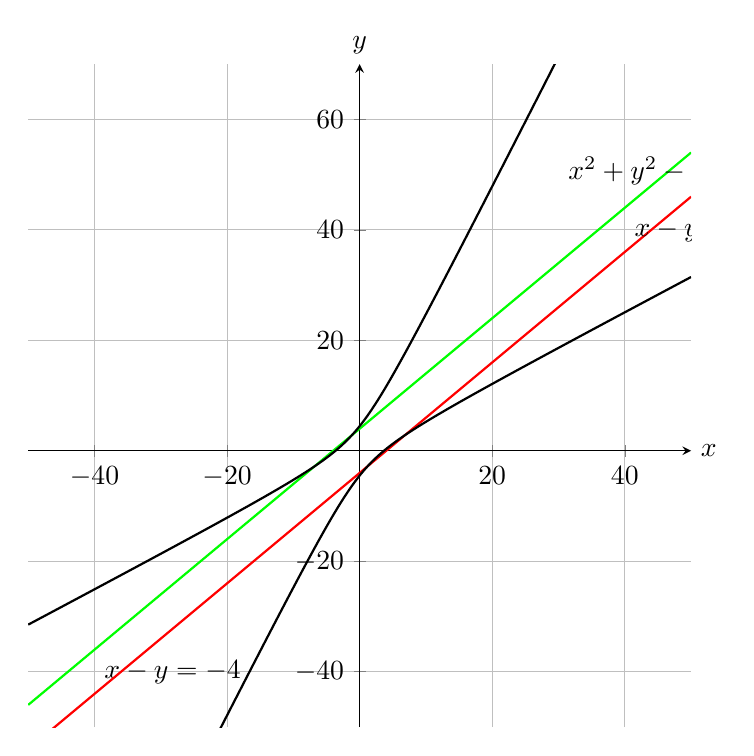
\begin{tikzpicture}
		\begin{axis}[
				axis lines=middle,
				grid=both,
				xmin=-50, xmax=50,
				ymin=-50, ymax=70,
				xlabel={$x$},
				ylabel={$y$},
				every axis x label/.style={at={(current axis.right of origin)}, anchor=west},
				every axis y label/.style={at={(current axis.above origin)}, anchor=south},
				width=10cm, height=10cm,
				samples=200,
				domain=-50:50
			]

			% Plot of x - y = -4
			\addplot[domain=-50:50, green, thick] {x + 4};
			\node[anchor=south west] at (axis cs:-40,-44) {$x - y = -4$};

			% Plot of x - y = 4
			\addplot[domain=-50:50, red, thick] {x - 4};
			\node[anchor=south west] at (axis cs:40,36) {$x - y = 4$};

			% Approximate implicit plot for x^2 + y^2 - 3xy - 20 = 0 using parametric plot
			\addplot[black, thick, samples=200, domain=-50:50]
			({x}, {(3*x + sqrt(3*x*x + 80))/2});
			\addplot[black, thick, samples=200, domain=-50:50]
			({x}, {(3*x - sqrt(3*x*x + 80))/2});
			\node[anchor=north west] at (axis cs:30,55) {$x^2 + y^2 - 3xy - 20 = 0$};

		\end{axis}
	\end{tikzpicture}
\end{center}


\section{Multiple Integration}

\nt{
	The integral
	\[
		\int_a^b f(x) \, dx = A
	\]
	represents the area under the curve \( f(x) \) from \( a \) to \( b \), where \( A \) can also be approximated as
	\[
		A \approx \sum_{i=1}^N f(x_i) \Delta x.
	\]
}

\nt{
To find the volume under a surface \( z = f(x, y) \) over a region \( R = [a, b] \times [c, d] \), we use the double integral
\[
	\iint_R f(x, y) \, dA.
\]
This can be approximated by summing over small subregions within \( R \):
\[
	\iint_R f(x, y) \, dA = \lim_{\Delta \to 0} \sum_{i=1}^m \sum_{j=1}^n f(x_i, y_j) \Delta x \, \Delta y.
\]
}

\thm{Continuity and Limits of Double Integrals}{
	If the limit
	\[
		\lim_{(x, y) \to (a, b)} f(x, y)
	\]
	exists for all points \( (a, b) \) in \( R \), then \( f(x, y) \) is continuous over \( R \), and the order of integration can be changed under Fubini's theorem.
}

\nt{
	Consider dividing \( R \) into \( n \) subregions, each with area \( \Delta A_{ij} \) and height \( f(x_i, y_j) \). Then, the volume \( V \) is approximated as
	\[
		V \approx \sum_{i=1}^m \sum_{j=1}^n f(x_i, y_j) \Delta x \, \Delta y,
	\]
	where \( n \) is the number of boxes in the \( x \)-direction and \( m \) is the number in the \( y \)-direction. Taking the limit as \( \Delta x, \Delta y \to 0 \) gives
	\[
		V = \iint_R f(x, y) \, dA.
	\]
}

\dfn{Double Integral Definition}{
The double integral of \( f(x, y) \) over \( R = [a, b] \times [c, d] \) is defined by
\[
	\iint_R f(x, y) \, dA = \lim_{n \to \infty} \sum_{i=1}^n \sum_{j=1}^n f(x_i, y_j) \Delta A_{ij}.
\]
}

\thm{Fubini's Theorem}{
	The order of integration does not affect the result of the double integral. Thus,
	\[
		\iint_R f(x, y) \, dA = \int_a^b \left( \int_c^d f(x, y) \, dy \right) dx = \int_c^d \left( \int_a^b f(x, y) \, dx \right) dy.
	\]
}

\ex{Example of Double Integral Calculation}{
Calculate the volume under \( f(x, y) = 4 + x + y^2 \) over the region \( R = [-1, 1] \times [0, 2] \):
\[
	\iint_R f(x, y) \, dA = \int_{-1}^1 \int_0^2 (4 + x + y^2) \, dy \, dx.
\]
Evaluating the inner integral with respect to \( y \),
\[
	\int_0^2 (4 + x + y^2) \, dy = 4y + xy + \frac{y^3}{3} \Big|_0^2 = 8 + 2x + \frac{8}{3}.
\]
Then, integrating with respect to \( x \),
\[
	\int_{-1}^1 \left( 8 + 2x + \frac{8}{3} \right) dx = \left( 8 + \frac{8}{3} \right) \cdot 2 = \frac{32}{3}.
\]
Thus, the volume \( V = \frac{32}{3} \).
}

\ex{Example: Integration Over a Rectangular Domain}{
	Evaluate
	\[
		\int_0^2 \int_0^1 \frac{x y}{1 + x^2} \, dx \, dy.
	\]

	Using substitution \( u = x^2 \) with \( du = 2x \, dx \), we find
	\[
		\int_0^2 \int_0^1 \frac{x y}{1 + x^2} \, dx \, dy = \int_0^2 y \left( \int_0^1 \frac{x}{1 + x^2} \, dx \right) dy = \int_0^2 y \left[ \frac{1}{2} \ln(1 + x^2) \right]_0^1 \, dy.
	\]
	Simplifying, we get
	\[
		V = \int_0^2 y \cdot \frac{\ln(2)}{2} \, dy = \frac{\ln(2)}{2} \int_0^2 y \, dy = \frac{\ln(2)}{2} \cdot \frac{y^2}{2} \Big|_0^2 = \ln(2).
	\]
}

\subsection{Non-Rectangular Domains}

\nt{
	Consider \( R = \{ (x, y) : a \leq x \leq b, g_1(x) \leq y \leq g_2(x) \} \), where the boundaries are given by functions \( y = g_1(x) \) and \( y = g_2(x) \).
}

\ex{Example: Non-Rectangular Domain Integration}{
	Suppose \( R = \{ (x, y) : -1 \leq x \leq 1, x^2 \leq y \leq 2 - x^2 \} \).
	We wish to evaluate
	\[
		\int_R (x+y) \, dA.
	\]
	We split \( R \) into two regions, \( R_1 \) and \( R_2 \), with bounds given by
	\[
		R_1 = \{ (x, y) : -1 \leq x \leq 1, x^2 \leq y \leq 2 - x^2 \}.
	\]
	Evaluating each integral, we obtain
	\[
		V = \int_{-1}^1 \left( \int_{x^2}^{2 - x^2} (x + y) \, dy \right) dx.
	\]

	On solving, we get
	\[
		V = \int_{-1}^1 \left( \int_{x^2}^{2 - x^2} (x + y) \, dy \right) dx = \ldots = \frac{8}{35}.
	\]
}

\begin{center}
	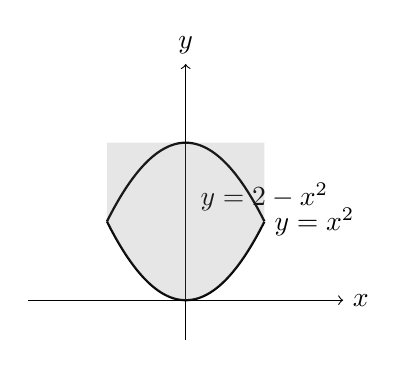
\begin{tikzpicture}
		% Define axes
		\draw[->] (-2,0) -- (2,0) node[right] {\( x \)};
		\draw[->] (0,-0.5) -- (0,3) node[above] {\( y \)};

		% Draw the curves
		\draw[thick, domain=-1:1, samples=100] plot (\x, {\x*\x}) node[right] {\( y = x^2 \)};
		\draw[thick, domain=-1:1, samples=100] plot (\x, {2 - \x*\x}) node[above] {\( y = 2 - x^2 \)};

		% Shade the region between curves
		\fill[gray, opacity=0.2] (-1,1) parabola bend (0,0) (1,1) -- (1,2) parabola bend (0,2) (-1,2) -- cycle;
	\end{tikzpicture}
\end{center}

\nt{
	When changing the order of integration, try dividing the region into smaller regions to make integration simpler.
}

\subsection{Volume Between Surfaces}

\nt{
	To find the volume of a sphere using double integrals, consider the surface
	\[
		x^2 + y^2 + z^2 = 1.
	\]
	Then \( z = \pm \sqrt{1 - x^2 - y^2} \), and we can set up the integral as
	\[
		V = 2 \iint_R \sqrt{1 - x^2 - y^2} \, dA,
	\]
	where \( R = \{ (x, y) : -1 \leq x \leq 1, -\sqrt{1 - x^2} \leq y \leq \sqrt{1 - x^2} \} \).
}

\begin{center}
	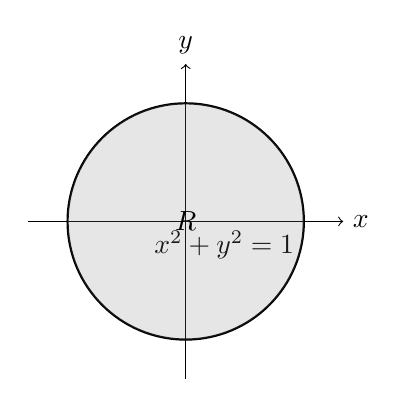
\begin{tikzpicture}
		% Define axes
		\draw[->] (-2,0) -- (2,0) node[right] {\( x \)};
		\draw[->] (0,-2) -- (0,2) node[above] {\( y \)};

		% Draw the circle for the sphere projection
		\draw[thick] (0,0) circle (1.5);
		\node[below left] at (1.5,0) {\( x^2 + y^2 = 1 \)};

		% Label the region
		\fill[gray, opacity=0.2] (0,0) circle (1.5);
		\node at (0,0) {\( R \)};
	\end{tikzpicture}
\end{center}

\ex{Example: Volume Between Surfaces}{
	Calculate the volume between the surfaces \( z = \sqrt{1 - x^2 - y^2} \) and \( z = -\sqrt{1 - x^2 - y^2} \):
	\[
		V = \iint_R \left( \sqrt{1 - x^2 - y^2} - (-\sqrt{1 - x^2 - y^2}) \right) \, dA = 2 \iint_R \sqrt{1 - x^2 - y^2} \, dA.
	\]
	Setting up the limits as before, we integrate over \( R \) to find the volume of the sphere.
}

\section{Applications of Double Integrals}

\subsection{Area of a Surface}

\dfn{Area of a Surface with Double integrals}{

	When calculating the area of a surface where the height of the surface in 3D space is constantly 1, the area of the surface is numerically equal to the volume under the surface. Thus, by setting the height \( f(x, y) = 1 \) over a given region \( R \), the area of \( R \) can be computed using a double integral, which effectively measures the "volume" under the constant surface.

	\[
		\text{Area of } R = \iint_R f(x, y) \, dA = \iint_R 1 \, dA
	\]
}

\ex{Example}{ Calculate the area of the region \( R = \{ (x, y) : x^2 + y^2 \leq 1 \} \), which is the unit disk in the \( xy \)-plane.

	\[
		\iint_R dA = \int_{-1}^1 \int_{-\sqrt{1 - x^2}}^{\sqrt{1 - x^2}} dy \, dx
	\]

	Calculating,
	\[
		= 2 \int_{-1}^1 \sqrt{1 - x^2} \, dx
	\]

	Using substitution, let \( x = \cos \theta \), we get:
	\[
		= 2 \int_0^\pi \sin^2 \theta \, d\theta = \pi
	\]

	Thus, the area of \( R \) is \( \pi \).
}


\begin{center}
	\begin{tikzpicture}
		\begin{axis}[
				width=12cm,
				height=12cm,
				view={135}{30},
				xlabel=$x$,
				ylabel=$y$,
				zlabel=$z$,
				zmin=0,
				xmin=-1.2, xmax=1.2,
				ymin=-1.2, ymax=1.2,
				grid=major,
				colormap/cool,
			]

			% Main cylinder surface
			\addplot3[
				surf,
				samples=50,
				domain=-1:1,
				y domain=-1:1,
				restrict expr to domain={x^2+y^2}{0:1},
				opacity=0.8,
			]
			{1};  % Height is constant at z=1

			% Bottom circle at z=0
			\addplot3[
				domain=0:360,
				samples=100,
				thick,
				color=black,
			]
			({cos(x)},{sin(x)},{0});

			% Top circle at z=1
			\addplot3[
				domain=0:360,
				samples=100,
				thick,
				color=black,
			]
			({cos(x)},{sin(x)},{1});

			% Cross-section curves
			\addplot3[
				color=red,
				thick,
				domain=-1:1,
				samples=50,
			]
			({x},{0},{1});

			\addplot3[
				color=blue,
				thick,
				domain=-1:1,
				samples=50,
			]
			({0},{x},{1});

			% Height indicator lines
			\foreach \x in {0.2,0.4,0.6,0.8} {
					\addplot3[
						dashed,
						color=gray,
					] coordinates {
							(\x,0,0)
							(\x,0,1)
						};
				}

			% Vertical lines at corners for better visibility
			\addplot3[thick, color=black] coordinates {(1,0,0) (1,0,1)};
			\addplot3[thick, color=black] coordinates {(-1,0,0) (-1,0,1)};
			\addplot3[thick, color=black] coordinates {(0,1,0) (0,1,1)};
			\addplot3[thick, color=black] coordinates {(0,-1,0) (0,-1,1)};

			% Add legend
			\addlegendentry{$z=1$ (Cylinder surface)}
			\addlegendentry{Region $R$}
			\addlegendentry{$x$-cross section}
			\addlegendentry{$y$-cross section}

		\end{axis}
	\end{tikzpicture}
\end{center}


\subsection{Average Value of a Function}

\dfn{Average Value of a Function}{
	The average value of a function \( f(x, y) \) over a region \( R \) is defined as the total value of \( f(x, y) \) over \( R \) divided by the area of \( R \). This can be expressed using double integrals as follows:

	\[
		\overline{f} = \frac{1}{\text{Area of } R} \iint_R f(x, y) \, dA = \frac{1}{\iint_R dA} \iint_R f(x, y) \, dA
	\]
}
\ex{Example}{
	Find the average value of \( f(x, y) = \sqrt{1 - x^2 - y^2} \) over the region \( R = \{ (x, y) : x^2 + y^2 \leq 1 \} \).

	First, calculate the area of \( R \):
	\[
		\text{Area of } R = \iint_R dA = \pi.
	\]

	Now, calculate the integral of \( f(x, y) \) over \( R \):
	\[
		\iint_R \sqrt{1 - x^2 - y^2} \, dA.
	\]

	Using polar coordinates, where \( x = r \cos \theta \) and \( y = r \sin \theta \), we have \( dA = r \, dr \, d\theta \):
	\[
		= \int_0^{2\pi} \int_0^1 \sqrt{1 - r^2} \cdot r \, dr \, d\theta.
	\]

	Breaking down the integral,
	\[
		= 2\pi \int_0^1 r \sqrt{1 - r^2} \, dr.
	\]

	Using the substitution \( u = 1 - r^2 \) (with \( du = -2r \, dr \)),
	\[
		= 2\pi \int_1^0 \sqrt{u} \cdot \left(-\frac{du}{2}\right) = \pi \int_0^1 \sqrt{u} \, du.
	\]

	Evaluating the integral,
	\[
		= \pi \int_0^1 u^{1/2} \, du = \pi \left[ \frac{u^{3/2}}{3/2} \right]_0^1 = \pi \cdot \frac{2}{3} = \frac{2\pi}{3}.
	\]

	Therefore, the average value of \( f(x, y) \) over \( R \) is
	\[
		\overline{f} = \frac{\frac{2\pi}{3}}{\pi} = \frac{2}{3}.
	\]
}


\begin{center}
	\begin{tikzpicture}
		\begin{axis}[
				width=12cm,
				height=12cm,
				view={135}{30},
				xlabel=$x$,
				ylabel=$y$,
				zlabel=$z$,
				zmin=0,
				xmin=-1.2, xmax=1.2,
				ymin=-1.2, ymax=1.2,
				grid=major,
				colormap/cool,
			]

			% Main surface plot
			\addplot3[
				surf,
				samples=50,
				domain=-1:1,
				y domain=-1:1,
				restrict expr to domain={x^2+y^2}{0:1},
				opacity=0.8,
			]
			{sqrt(1-x^2-y^2)};

			% Boundary circle at z=0
			\addplot3[
				domain=0:360,
				samples=100,
				thick,
				color=black,
			]
			({cos(x)},{sin(x)},{0});

			\addplot3[
				color=red,
				thick,
				domain=-1:1,
				samples=50,
			]
			({x},{0},{sqrt(max(0,1-x^2))});

			\addplot3[
				color=blue,
				thick,
				domain=-1:1,
				samples=50,
			]
			({0},{x},{sqrt(max(0,1-x^2))});

			% Height indicator lines
			\foreach \x in {0.2,0.4,0.6,0.8} {
					\addplot3[
						dashed,
						color=gray,
					] coordinates {
							(\x,0,0)
							(\x,0,{sqrt(1-\x^2)})
						};
				}

			% Add legend
			\addlegendentry{$f(x,y)=\sqrt{1-x^2-y^2}$}
			\addlegendentry{Region $R$}
			\addlegendentry{$x$-cross section}
			\addlegendentry{$y$-cross section}

		\end{axis}
	\end{tikzpicture}
\end{center}

\section{Derivation of Triple Integrals through Riemann Sums}

To derive the concept of a triple integral, we start by considering a bounded, three-dimensional region \( D \subset \mathbb{R}^3 \) over which we wish to integrate a continuous function \( f(x, y, z) \). The idea is to approximate the "volume" under the surface defined by \( f(x, y, z) \) over \( D \) by partitioning \( D \) into smaller subregions, summing up values of \( f \) at chosen points within these subregions, and then taking the limit as the partitions become finer.

\subsection{Partitioning the Region}

1. Let \( D \) be divided into \( n \times m \times l \) subregions, each of volume \( \Delta V_{ijk} = \Delta x_i \Delta y_j \Delta z_k \), where:
\[
	\Delta x_i = x_{i+1} - x_i, \quad \Delta y_j = y_{j+1} - y_j, \quad \Delta z_k = z_{k+1} - z_k
\]

2. In each subregion, choose a point \( (x_i^*, y_j^*, z_k^*) \) where \( f \) will be evaluated. The function value at each of these points, \( f(x_i^*, y_j^*, z_k^*) \), approximates the "height" over the corresponding volume element.

\subsection{Forming the Riemann Sum}

With these chosen points and partition, the Riemann sum for \( f \) over the region \( D \) is given by:
\[
	\sum_{i=1}^n \sum_{j=1}^m \sum_{k=1}^l f(x_i^*, y_j^*, z_k^*) \Delta x_i \Delta y_j \Delta z_k.
\]

As the partitions become finer, i.e., \( \Delta x_i, \Delta y_j, \Delta z_k \to 0 \) for all \( i, j, k \), the sum approaches the exact "volume" under \( f \) over \( D \), which we denote as the triple integral:
\[
	\iiint_D f(x, y, z) \, dV = \lim_{n, m, l \to \infty} \sum_{i=1}^n \sum_{j=1}^m \sum_{k=1}^l f(x_i^*, y_j^*, z_k^*) \Delta x_i \Delta y_j \Delta z_k.
\]

Thus, the triple integral represents the limit of the Riemann sum as the volume elements \( \Delta V_{ijk} \) become infinitesimally small.

\section{Triple Integrals Intuitions and Applications}

\[
	\int f(x) \, dx \rightarrow \text{Area} \quad \int\int f(x,y) \, dA \rightarrow \text{Volume under } f(x,y)
\]
\[
	\iiint f(x,y,z) \, dV \rightarrow \text{Volume under solid } w = f(x,y,z)
\]

\subsection{Integrals Represent Products}
\[
	\text{Examples:}
\]
\[
	\text{Length } = F = P \cdot A \quad \Rightarrow \quad \iint_R P(x,y) \, dA
\]
\[
	\text{Mass } = \rho \cdot V \quad \Rightarrow \quad m = \iiint_D \rho(x,y,z) \, dV
\]

\ex{Mass of a Rock}{
	Suppose a rock with uniform density $\rho$ and volume $V$. Then
	\[
		m = \rho V
	\]
	If $\rho$ is non-uniform, how do you find the mass?

	Suppose $\rho(x,y,z)$ is given by $p(x,y,z)$ over the support of $D$, then
	\[
		m = \iiint_D p(x,y,z) \, dV
	\]
	where \( D \subseteq \mathbb{R}^3 \) is the region occupied by the rock.
}
\ex{Volume}{
	Note $A \subseteq \mathbb{R}^2$, then
	\[
		\text{Volume of } D \text{ in } \mathbb{R}^3
	\]
	is
	\[
		V = \iiint_D \, dV
	\]
}

\ex{Example 3: Probability Densities}{
	Let $x, y, z$ be variables representing random quantities. You can find $f(x,y,z)$ called a Probability Density Function (P.D.F.) where
	\[
		P((x,y,z) \in D) = \iiint_D f(x,y,z) \, dV
	\]
}
\dfn{Bounds of Integration for triple integrals}{
	Suppose \( D = \{ (x,y,z) : a \leq x \leq b, \, g(x) \leq y \leq h(x), \, G(x,y) \leq z \leq H(x,y) \} \),
	where the bounds of \( y \) depend on \( x \) and the bounds of \( z \) depend on \( x \) and \( y \).

	Then
	\[
		V = \iiint_D f(x,y,z) \, dV = \int_a^b \int_{g(x)}^{h(x)} \int_{G(x,y)}^{H(x,y)} f(x,y,z) \, dz \, dy \, dx
	\]
}

\ex{PDF in 3 Continous Random Variables}{
Three customers wait \( x, y, z \) minutes.

\[
	f(x,y,z) = \begin{cases}
		10^3 e^{-(x+y+z)} \cdot \frac{1}{10} & \text{if } x, y, z \geq 0 \\
		0                                    & \text{otherwise}
	\end{cases}
\]

\paragraph{(1) Probability that \( (x,y,z) \in D \):}
\[
	P((x,y,z) \in D) = \iiint_D 10^3 e^{-(x+y+z)} \cdot \frac{1}{10} \, dV
\]

\paragraph{(2) Probability that customers wait at most 5 minutes:}
\[
	D = [0,5] \times [0,5] \times [0,5]
\]
\[
	P = \iiint_D 10^3 e^{-(x+y+z)} \cdot \frac{1}{10} \, dx \, dy \, dz = 0.061 = 6.1\%
\]

\paragraph{(3) Probability that \( 0 \leq x \leq y \leq z \leq 20 \):}
Define
\[
	P = \{ (x,y,z) : 0 \leq x \leq y \leq z \leq 20 \}
\]
1. Find the domain of \( x \) in \( D \):
\[
	0 \leq x \leq 20
\]
2. Fix some \( x = x_0 \), define \( R = \{ (y,z) : 0 \leq x_0 \leq y \leq 20 \} \).
3. Marginalize \( y \) in \( R \):
\[
	x \leq y \leq 20
\]
4. Marginalize \( z \) in \( R \):
\[
	y \leq z \leq 20
\]

Thus,
\[
	D = [0,20] \times [x,20] \times [y,20]
\]
\[
	P = \int_0^{20} \int_x^{20} \int_y^{20} 10^3 e^{-(x+y+z)} \cdot \frac{1}{10} \, dz \, dy \, dx
\]
}

\thm{Fubini’s Theorem Extended to Triple Integrals}{
Fubini’s Theorem allows us to evaluate triple integrals as iterated integrals by integrating one variable at a time. If \( f(x,y,z) \) is continuous on a rectangular region \( D = [a,b] \times [c,d] \times [e,f] \), then
\[
	\iiint_D f(x,y,z) \, dV = \int_a^b \int_c^d \int_e^f f(x,y,z) \, dz \, dy \, dx.
\]

This can also be rearranged in different orders of integration:
\[
	\iiint_D f(x,y,z) \, dV = \int_c^d \int_a^b \int_e^f f(x,y,z) \, dx \, dz \, dy,
\]
and similarly for other orders, depending on the bounds and convenience for computation.
}


\end{document}